\chapter{度规、膨胀与最初的宇宙学}

在前一讲的末尾，我们已经得到了一个洛伦兹不变的波动方程，并正准备把麦克斯韦方程组写成时空形式。现在，在转向引力之前，一位听众的提问提供了一个有用的警示：对称性本身究竟能决定一个物理理论的多少内容？答案是明确的：能决定很多，但并非全部。洛伦兹不变性是对可能定律的一个强有力的筛选条件。它并不能替代其余物理假设，也不能替代实验。

\section{对称性所不能决定的内容}

\begin{classroomqa}
\audiencequestion{一旦已知电场和磁场在洛伦兹变换下会一起变换，麦克斯韦方程组是否仅由相对论就能推出？}
\lecturerresponse{不能。相对论约束了这些方程的形式，但其构造还使用了方程的线性性、其导数阶数之低、场变换的方式以及实验信息。若没有这些额外要素，许多洛伦兹协变的场方程仍将是可能的。}
\end{classroomqa}

在开篇讨论中，这些额外假设里最重要的是线性性。如果\(A(x,t)\)是某个线性场方程的解，那么对任意常数\(\lambda\)，\(\lambda A(x,t)\)也是解。如果\(A\)和\(B\)是解，那么\begin{equation}
  C(x,t)=A(x,t)+B(x,t).
  \label{eq:superposition}
\end{equation}也是解。这就是叠加原理。两列无源电磁波可以彼此交叉而保持原样。它们不会像实物那样直接碰撞。它们可以通过带电物质间接相互作用，因为每一列波都会推动电荷，而运动电荷会辐射，但真空中的场方程本身是线性的。

\begin{figure}[H]
\centering
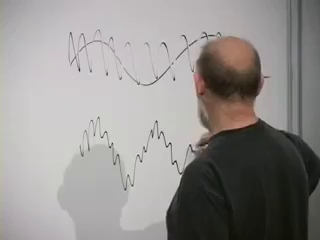
\includegraphics[width=0.64\textwidth]{lecture_08_figure_01.png}
\caption{讨论叠加原理时黑板上的两个波剖面。它们的和仍然是一列允许的无源波。}
\lectureframe{00:05:30}
\end{figure}

谐振子使这套代数变得清楚明了。假设\begin{equation}
  m\ddot x=-kx.
  \label{eq:linear-oscillator}
\end{equation}。如果\(x_1\)和\(x_2\)解\eqref{eq:linear-oscillator}，那么\begin{equation}
  m(\ddot x_1+\ddot x_2)
  =-k(x_1+x_2),
\end{equation}，所以\(x_1+x_2\)是解。然而，加上一个非线性项后，\begin{equation}
  m\ddot x=-kx+p x^2,
  \label{eq:nonlinear-oscillator}
\end{equation}，其和就不再成立：\begin{equation}
  (x_1+x_2)^2=x_1^2+x_2^2+2x_1x_2.
\end{equation}。交叉项\(2x_1x_2\)在两个分开的方程中没有对应项。这两种运动现在会相互影响。

\begin{figure}[H]
\centering
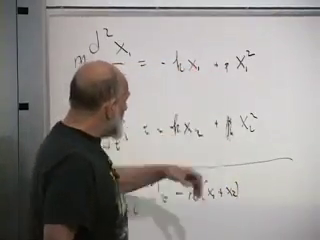
\includegraphics[width=0.73\textwidth]{lecture_08_figure_02.png}
\caption{将分开的振子方程与其和的方程相比较。二次项暴露出破坏叠加原理的额外交叉项。}
\lectureframe{00:10:10}
\end{figure}

这个例子确定了将在整个宇宙学讨论中始终有效的方法论要点。对称性告诉我们哪些量可以组合，以及哪些方程是允许的。动力学和观测则告诉我们自然界使用的是哪一个允许的方程。

\section{作为几何的间隔}

现在我们离开电磁学，走一条短路线进入广义相对论和宇宙学。起始对象是相邻事件之间的间隔。用一个四维坐标\(x^\mu\)标记一个事件，并用\(x^\mu+dx^\mu\)标记一个邻近事件。在惯性笛卡儿坐标中，取\(c=1\)和\((+,-,-,-)\)约定，\begin{equation}
  d\tau^2
  =dt^2-dx^2-dy^2-dz^2
  =dx^\mu dx_\mu
  =\eta_{\mu\nu}\,dx^\mu dx^\nu.
  \label{eq:minkowski-interval}
\end{equation}。不变量是量\(d\tau^2\)，而不是任何一个坐标差。洛伦兹变换会改变\(dt,dx,dy,dz\)，同时保持这个二次组合不变。因此，狭义相对论可以被解读为闵可夫斯基时空的几何。

\begin{figure}[H]
\centering
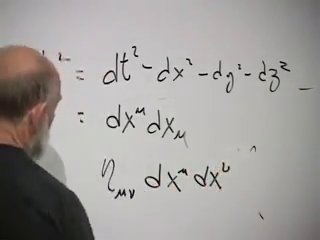
\includegraphics[width=0.72\textwidth]{lecture_08_figure_03.png}
\caption{闵可夫斯基间隔依次用分量、缩并指标和度规张量记号写出。}
\lectureframe{00:14:50}
\end{figure}

\eqref{eq:minkowski-interval}的简单性取决于坐标。即使是一个平坦平面，如果我们不明智地给它标记坐标，也会获得不熟悉的系数。设\(x\)以厘米为单位测量，而\(y\)以米为单位测量。对于一个物理位移，\begin{equation}
  ds^2=dx^2+\left(\frac{dy}{100}\right)^2
      =dx^2+10^{-4}dy^2.
  \label{eq:mixed-units}
\end{equation}。因子\(10^{-4}\)与曲率毫无关系。它只是在单位之间进行换算。

\begin{figure}[H]
\centering
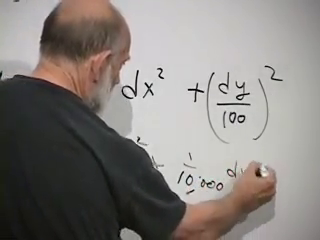
\includegraphics[width=0.59\textwidth]{lecture_08_figure_04.png}
\caption{一个平坦平面，一个轴用厘米描述，另一个轴用米描述。不相等的度规系数编码的是单位，而不是曲率。}
\lectureframe{00:20:10}
\end{figure}

斜坐标会添加一个混合项。在二维中，最一般的局部二次型可以写成\begin{align}
  ds^2
  &=a_{11}\,dx^2+a_{12}\,dx\,dy\notag\\
  &\quad+a_{21}\,dy\,dx+a_{22}\,dy^2,
  \qquad a_{12}=a_{21}.
  \label{eq:quadratic-form}
\end{align}。因为普通微分可交换，\(dx\,dy=dy\,dx\)，所以只有系数阵列的对称部分有贡献。我们把系数收集到矩阵\begin{equation}
  g=
  \begin{pmatrix}
    a_{11} & a_{12}\\
    a_{21} & a_{22}
  \end{pmatrix}.
  \label{eq:metric-matrix}
\end{equation}中。这个矩阵就是\emph{度规}。它是把坐标差转换为物理间隔的局部规则。

\begin{figure}[H]
\centering
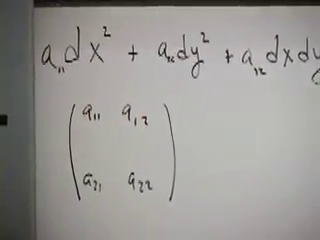
\includegraphics[width=0.71\textwidth]{lecture_08_figure_05.png}
\caption{二次微分形式及其对称的\(2\times2\)系数矩阵，此时该矩阵被认定为度规。}
\lectureframe{00:24:07}
\end{figure}

均匀的矩形或斜交网格给出常系数。如果坐标线弯曲、聚拢或散开，那么即使底层曲面仍然是平的，这些系数也会变成位置的函数。一般的时空记号是
\begin{equation}
  ds^2=g_{\mu\nu}(x)\,dx^\mu dx^\nu.
  \label{eq:general-metric}
\end{equation}

\begin{figure}[H]
\centering
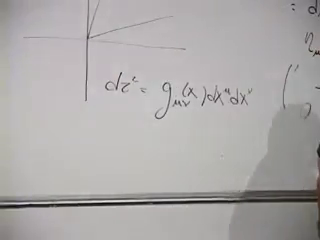
\includegraphics[width=0.66\textwidth]{lecture_08_figure_06.png}
\caption{允许坐标网格逐点变化后的一般位置依赖度规。}
\lectureframe{00:28:10}
\end{figure}

在指定坐标系中知道\(g_{\mu\nu}\)，就确定了局部的距离、时间和角度，从而确定了几何。反之则不唯一：一种几何有无穷多种坐标描述，因此有无穷多组由坐标变换相联系的系数函数阵列。

\section{坐标复杂性与内禀曲率}

我们现在必须把复杂的度规与弯曲的空间区分开来。把一张纸卷成圆柱而不拉伸它。它在房间中的外观改变了，但在纸内测得的所有距离都保持不变。一个被限制在纸上的生物无法通过任何内禀测量探测到这种弯曲。那是外在弯曲，不是这里所说的曲率。

半球则不同。不拉伸、不撕裂、不压缩它，就无法把它压平。地球的平面地图必然扭曲距离、面积、角度或它们的某种组合。这种阻碍是内禀的，无需看向周围维度就能探测到。

极坐标给出了不可或缺的平坦反例。在平面上，无穷小径向位移的长度为\(dr\)，而在半径\(r\)处的角位移\(d\theta\)的长度为\(r\,d\theta\)。因此
\begin{equation}
  ds^2=dr^2+r^2d\theta^2,
  \qquad
  g_{\text{polar}}=
  \begin{pmatrix}
    1&0\\
    0&r^2
  \end{pmatrix}.
  \label{eq:polar-metric}
\end{equation}
系数\(r^2\)在整个平面上变化，然而平面是平的。变量变换
\begin{equation}
  x=r\cos\theta,\qquad y=r\sin\theta
\end{equation}
又回到常度规\(ds^2=dx^2+dy^2\)。

\begin{figure}[H]
\centering
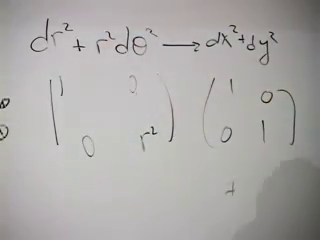
\includegraphics[width=0.70\textwidth]{lecture_08_figure_07.png}
\caption{极坐标度规及其向笛卡尔度规的回归。左边位置依赖的矩阵仍然描述一个平坦的平面。}
\lectureframe{00:39:20}
\end{figure}

\begin{classroomqa}
\audiencequestion{极坐标中的角距离是否应包含一个正弦？}
\lecturerresponse{在平面上不是。那里的弧长是\(r\,d\theta\)。正弦出现在球面上，那里一条纬线圆的半径为\(R\sin\theta\)。}
\end{classroomqa}

取半径为\(R\)的球面。设\(\theta\)为从北极量起的极角，\(\phi\)为方位角。经向一步的长度为\(R\,d\theta\)。在极角\(\theta\)处，纬圈的半径为\(R\sin\theta\)，因此方位角一步的长度为
\(R\sin\theta\,d\phi\)。局部勾股定理给出
\begin{align}
  ds^2
  &=R^2\left(d\theta^2+\sin^2\theta\,d\phi^2\right),
  \label{eq:sphere-metric}\\
  g_{\text{sphere}}=
  &\begin{pmatrix}
    R^2&0\\
    0&R^2\sin^2\theta
  \end{pmatrix}.
\end{align}

\begin{figure}[H]
\centering
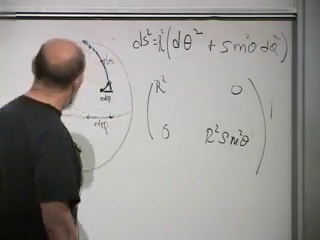
\includegraphics[width=0.72\textwidth]{lecture_08_figure_08.png}
\caption{球面、其角向线元以及相应的度规矩阵。\(\sin^2\theta\)因子记录了纬圈的收缩。}
\lectureframe{00:45:15}
\end{figure}

\begin{figure}[H]
\centering
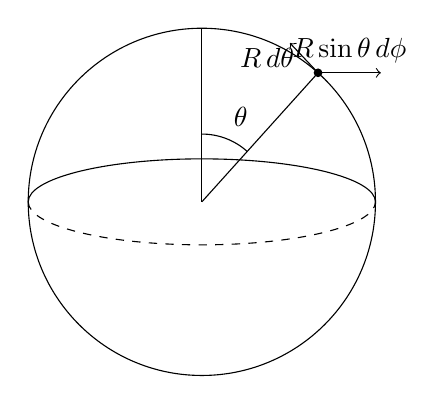
\begin{tikzpicture}[scale=1.05]
  \draw (0,0) circle (2.1);
  \draw[dashed] (-2.1,0) arc (180:360:2.1 and 0.52);
  \draw (2.1,0) arc (0:180:2.1 and 0.52);
  \coordinate (P) at (48:2.1);
  \fill (P) circle (1.5pt);
  \draw (0,0) -- (0,2.1);
  \draw (0,0) -- (P);
  \draw (0,0.82) arc (90:48:0.82);
  \node at (0.47,1.03) {\(\theta\)};
  \draw[->] (P) -- ++(-0.34,0.36)
    node[midway,left] {\(R\,d\theta\)};
  \draw[->] (P) -- ++(0.76,0)
    node[midway,above] {\(R\sin\theta\,d\phi\)};
\end{tikzpicture}
\caption{用于得到\eqref{eq:sphere-metric}的局部微分腿的清晰重构。}
\end{figure}

没有任何整体坐标变换能把\eqref{eq:sphere-metric}变成常欧几里得矩阵。一个二维观测者可以内禀地发现这一点：由测地线构成的足够大的三角形，其内角和大于\(180^\circ\)。因此我们得到了有用的判据。变系数本身并不蕴含曲率。曲率是找不到使度规在所考虑区域内处处为常数的坐标这一阻碍。

\section{从弯曲时空到宇宙学}

广义相对论允许时空本身具有这种内禀曲率。位置依赖的\(g_{\mu\nu}\)可能仍然只是坐标的产物，如在极坐标中那样，但在真正弯曲的时空中，没有任何坐标变换能在整体上消除这种变化。

\begin{figure}[H]
\centering
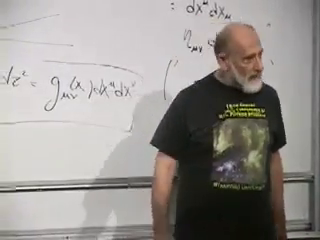
\includegraphics[width=0.70\textwidth]{lecture_08_figure_09.png}
\caption{从特殊坐标例子到一般时空线元\(ds^2=g_{\mu\nu}(x)dx^\mu dx^\nu\)的过渡。}
\lectureframe{00:48:40}
\end{figure}

我们不会尝试爱因斯坦方程的全部机器。相反，我们把注意力限制在适合宇宙学的几何上：空间在足够大的尺度上被取为均匀的，而几何可以随时间变化。均匀意味着没有任何位置与其他位置相区别。它并不意味着平坦：球面上的每一点都等价，然而球面是弯曲的。它也不意味着在每个尺度上都无特征。

\begin{classroomqa}
\audiencequestion{如果星系会形成星系团、片状结构和纤维状结构，宇宙怎么可能是均匀的？}
\lecturerresponse{这一论断涉及的是粗粒化尺度。恒星、星系和星系团是强烈非均匀的。当把横跨数亿光年的区域相互比较时，这些结构在平均意义上趋于均匀分布。宇宙学原理是一种经验性的工作假设，而不是逻辑上的必然；足够大的系统性差异，包括宇宙背景中的方向性差异，都可能证伪它。}
\end{classroomqa}

本讲的第二个大尺度假设是空间平坦性。在固定的宇宙时刻，足够大的三角形看起来是欧几里得的：其内角之和为\(180^\circ\)。这是关于三维空间几何的陈述，尚未涉及四维时空的曲率。

\begin{classroomqa}
\audiencequestion{对于相隔宇宙学距离的点，同时性意味着什么？毕竟它们的光在不同时刻到达我们这里。}
\lecturerresponse{我们无法在遥远星系之间放置量杆，也无法瞬时地检视它们。我们是在较晚的时候接收到信号，并在某个时空模型内重建发射事件的几何。这一程序是间接的，但天文学中的许多几何测量也是如此。平坦性意味着，在所考察的尺度上，重建出的大三角形没有可探测到的角盈余或角亏损。}
\end{classroomqa}

\section{共动坐标与尺度因子}

想象一张笛卡尔网格被画在星系的大尺度流动之上。随着网格膨胀，每个星系保持其坐标标签不变。这个标签不是以米为单位的距离，而是一个地址。一个随时间变化的转换因子把坐标间隔变成物理间隔。

\begin{figure}[H]
\centering
\begin{tikzpicture}[>=Latex,scale=0.86]
  \foreach \x in {0,0.65,1.3,1.95,2.6} {
    \draw[gray!65] (\x,0) -- (\x,2.2);
  }
  \foreach \y in {0,0.55,1.1,1.65,2.2} {
    \draw[gray!65] (0,\y) -- (2.6,\y);
  }
  \fill[blue!65!black] (0.65,0.55) circle (2pt);
  \fill[red!70!black] (1.95,1.65) circle (2pt);
  \node[below] at (1.3,-0.2) {comoving labels at \(t_1\)};
  \draw[->,very thick] (3.0,1.1) -- (4.0,1.1)
    node[midway,above] {\(a(t)\) grows};
  \foreach \x in {4.4,5.5,6.6,7.7,8.8} {
    \draw[gray!65] (\x,0) -- (\x,2.2);
  }
  \foreach \y in {0,0.55,1.1,1.65,2.2} {
    \draw[gray!65] (4.4,\y) -- (8.8,\y);
  }
  \fill[blue!65!black] (5.5,0.55) circle (2pt);
  \fill[red!70!black] (7.7,1.65) circle (2pt);
  \node[below] at (6.6,-0.2) {same labels at \(t_2\)};
\end{tikzpicture}
\caption{共动地址保持固定，而坐标网格的物理间距在增大。}
\end{figure}

空间均匀性要求：在给定时刻，处处都有相同的转换因子。空间平坦性则允许度规的空间部分取笛卡尔形式。由此得到的线元为
\begin{equation}
  d\tau^2
  =dt^2-a^2(t)\left(dx^2+dy^2+dz^2\right).
  \label{eq:flrw-flat}
\end{equation}
这就是共动坐标下空间平坦的均匀宇宙学度规。我们可以选择让\(x,y,z\)无量纲，并赋予\(a(t)\)长度的单位。另一种约定可以把量纲放进坐标中，使\(a\)无量纲；只有乘积才是有意义的。

\begin{figure}[H]
\centering
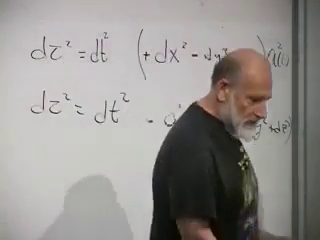
\includegraphics[width=0.76\textwidth]{lecture_08_figure_10.png}
\caption{黑板上写出的空间平坦宇宙学度规，其中共同的因子\(a^2(t)\)乘在全部三个空间方向上。}
\lectureframe{01:03:15}
\end{figure}

如果\(a\)是常数，我们就可以通过重新标度\(x,y,z\)把它吸收掉，而\eqref{eq:flrw-flat}就会是换用不同单位的普通闵可夫斯基时空。它的时间依赖才是非平凡之处。

\begin{classroomqa}
\audiencequestion{如果坐标网格在膨胀，为什么米尺、原子和星系不随之膨胀？}
\lecturerresponse{度规描述的是宇宙的平均流动，而不是一种迫使每个束缚系统都跟随它的力。电磁力把米尺和原子束缚在一起；自引力把星系束缚在一起。在小尺度上，这些束缚效应压倒了极其微弱的背景膨胀。近邻星系也可以偏离哈勃流：仙女座星系正被银河系吸引。对星系束缚的详细研究表明，仅有可见物质是不够的，这是支持暗物质的论据之一。}
\end{classroomqa}

\begin{classroomqa}
\audiencequestion{为什么尺度因子本身不是一种把星系推开的力？}
\lecturerresponse{在目前的约定下，它具有长度的量纲，而不是力的量纲。想想向上发射的一颗炮弹。一旦发射出去，它的向外运动就是惯性的；引力通过减小其速度或把它拉回来来改变这种运动。同样，膨胀是一种运动状态。动力学问题是引力和其它源如何改变\(\dot a\)和\(\ddot a\)，而不是需要什么力来维持\(a\)的运动。}
\end{classroomqa}

过去的预期是，吸引性引力应当使膨胀减速。到本讲之时，天文证据已经表明，近期的膨胀反而在加速，这意味着完整的动力学所包含的内容不止普通的吸引性物质。我们把这个问题推迟到几何框架稳固之后再讨论。

\section{哈勃定律}

取两个共动星系，其固定坐标间隔为
\(\Delta x\)。在共同的宇宙时刻，它们的物理距离为
\begin{equation}
  D(t)=a(t)\,\Delta x.
  \label{eq:physical-distance}
\end{equation}
在保持共动标签固定的情况下求导：
\begin{align}
  V(t)
    &=\dot D(t)
      =\dot a(t)\,\Delta x \nonumber\\
    &=\frac{\dot a(t)}{a(t)}D(t).
  \label{eq:hubble-derivation}
\end{align}
定义
\begin{equation}
  H(t)=\frac{\dot a(t)}{a(t)}.
  \label{eq:hubble-parameter}
\end{equation}
于是
\begin{equation}
  V(t)=H(t)D(t).
  \label{eq:hubble-law}
\end{equation}
在某一宇宙时刻，同一个\(H(t)\)处处适用；否则空间就不会是均匀的。退行速度与距离成正比，因为共动网格中的每一个间隔都以相同的分数速率被拉伸。

\begin{figure}[H]
\centering
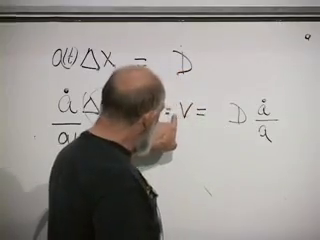
\includegraphics[width=0.73\textwidth]{lecture_08_figure_11.png}
\caption{物理距离\(D=a\Delta x\)及其时间导数，在通向\(V=(\dot a/a)D\)的过程中。}
\lectureframe{01:16:45}
\end{figure}

\begin{classroomqa}
\audiencequestion{对于一个遥远的星系，哈勃参数应当用现在的值，还是用所观测到的光发出时的值来求？}
\lecturerresponse{用所描述的那个时期的值。来自遥远星系的光报告的是较早的膨胀值。严肃的分析必须考虑\(H\)的时间依赖性；处处代入今天的值只是一种局部近似。}
\end{classroomqa}

\begin{classroomqa}
\audiencequestion{在\(D=a\Delta x\)中，单位存在于何处？}
\lecturerresponse{一个方便的选择是把共动标签\(\Delta x\)视为无量纲，而让\(a\)带有长度量纲。相反的记账方式也是可能的。无论哪种方式，\(H=\dot a/a\)都具有时间的倒数量纲。}
\end{classroomqa}

\section{膨胀坐标中的光}

光沿零路径传播。沿这样的路径，固有时间隔为零：
\begin{equation}
  d\tau^2=0.
\end{equation}

\begin{classroomqa}
\audiencequestion{为什么光的间隔为零？}
\lecturerresponse{这就是相对论中光线之所以为光线的定义性几何。每一个局部自由下落的观测者都测得光以\(c=1\)运动，因此局部地有\(dt^2=d\ell^2\)，时空间隔为零。这并不意味着接收光的观测者没有坐标时间流逝。}
\end{classroomqa}

对于只沿\(x\)方向运动的光线，
\begin{equation}
  0=dt^2-a^2(t)\,dx^2.
\end{equation}
选择朝\(x\)增大的方向运动的那条光线，
\begin{equation}
  dt=a(t)\,dx,
  \qquad
  dx=\frac{dt}{a(t)},
  \qquad
  \frac{dx}{dt}=\frac{1}{a(t)}.
  \label{eq:null-ray}
\end{equation}

\begin{figure}[H]
\centering
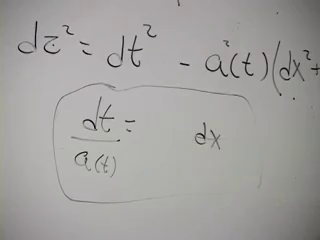
\includegraphics[width=0.64\textwidth]{lecture_08_figure_12.png}
\caption{膨胀度规中的零条件以及由此得到的共动光线方程\(dx=dt/a(t)\)。}
\lectureframe{01:23:45}
\end{figure}

坐标速度\(dx/dt\)随尺度因子增大而减小。这并不意味着光在局部变慢。一个单位的共动坐标距离代表越来越大的物理距离，因此坐标速度的数值发生变化，而每一次局部测量仍然给出\(c=1\)。

\section{为什么时间依赖性很重要}

现在，核心的几何问题不可避免：\(a(t)\)如何变化？类比于一个在某时刻位置已知的抛射体。它未来的轨迹需要运动方程。在宇宙学中，引力动力学将提供关于\(a(t)\)的方程。

\begin{classroomqa}
\audiencequestion{为什么要特别追问\(a(t)\)是否随时间变化，而不去同样合理地追问例如电子电荷是否随时间变化？}
\lecturerresponse{并不存在逻辑上的等级之分。电子电荷若被测出变化，那将是极其重要的。我们聚焦于\(a(t)\)，是因为观测已经告诉我们宇宙间隔在变化，而电子电荷看起来是恒定的。从几何上看，一个恒定的\(a\)可以通过改变空间单位而被移除，并留下平坦时空；一个随时间变化的\(a\)则不能以那种方式被移除。}
\end{classroomqa}

在测量遥远星系的退行之前，需要这个几何框架来说明所测量的究竟是什么。在最粗略的层面上，一个已知光度的源会因距离而显得更暗，因为它的光散布在更大的面积上；而已知原子谱线的位移给出红移，从而给出退行指标。哈勃把距离估计与红移结合起来，揭示了正比关系
\eqref{eq:hubble-law}，尽管该系数早期的数值有实质性错误。现代的距离阶梯和相对论性光传播计算要精细得多，但概念上的配对仍然是距离加红移。

\section{哈勃时间与年龄估计}

哈勃定律中隐藏着一个简单的估计。冻结一个星系当前的退行速度，并让运动均匀地反向进行。闭合其当前距离所需的时间将是
\begin{equation}
  t=\frac{D}{V}.
\end{equation}
利用\(V=HD\)，
\begin{equation}
  t=\frac{D}{HD}=\frac{1}{H}.
  \label{eq:hubble-time}
\end{equation}
距离被消去，因此每一对共动星系都给出相同的粗略时间。Susskind在此抓住并纠正了一个容易犯的措辞错误。假设并不是\(H\)保持恒定。而是把那个特定的退行速度当作恒定的一样向后外推。

\begin{figure}[H]
\centering
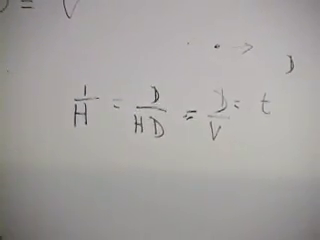
\includegraphics[width=0.66\textwidth]{lecture_08_figure_13.png}
\caption{哈勃时间估计 \(H^{-1}=D/(HD)=D/V\)，其中距离在反向外推中相消。}
\lectureframe{01:33:45}
\end{figure}

因此，逆哈勃参数是一个时间尺度，并不自动等于宇宙的精确年龄。在纯减速、物质主导的图像中，将当前速度反向，并让引力把星系拉回到一起。它们相遇的时间比在匀速情况下更早，所以当前的 \(H^{-1}\) 高估了年龄。讲座引用了一个更精确的年龄，约为 \(13.5\) 亿年，接近哈勃时间但并不完全相同。

\begin{classroomqa}
\audiencequestion{如果我们的星系内部没有哈勃膨胀，那么把所有星系反向运行直到它们坍缩意味着什么？}
\lecturerresponse{均匀描述最终不再能分辨束缚结构的真实历史。在时间正向上，小涨落通过引力增长为星系和星系团。字面意义上的倒放电影将要求每一个微观运动都反向，并且熵减少；仅仅反转平均哈勃流并不能撤销结构形成。反向外推是一种粗略的宇宙学估计，而不是每颗恒星沿其路径回溯的影片。}
\end{classroomqa}

\begin{classroomqa}
\audiencequestion{实验能否区分星系际距离在膨胀与尺子在收缩？}
\lecturerresponse{只有无量纲比值是可观测的。所测量到的是星系之间的距离除以原子或实验室长度标准后增大。我们习惯上保持原子和分子物理的参数固定，并说宇宙在膨胀。也可以选择星系际间距作为标准，而把原子、质子和米尺描述为在收缩。该比值的物理将保持不变。}
\end{classroomqa}

这种约定是自然的，因为尺子由原子构成，而其大小由那些看起来恒定的参数控制。一米归根结底是大量微观长度的总和。保持这些微观标准固定，就得到熟悉的说法：\(a(t)\) 在增长。

\begin{classroomqa}
\audiencequestion{\eqref{eq:flrw-flat} 是唯一与空间均匀性和平坦性相容的度规吗？}
\lecturerresponse{只在坐标变换的意义下唯一。精确的说法是，在这些假设下，并适当选择宇宙时间和共动空间坐标，度规可以被化为这种形式。另一个坐标系可能使同一个时空看起来相当不同。}
\end{classroomqa}

\begin{classroomqa}
\audiencequestion{当反向分离达到零时，哈勃定律也给出零速度。这会阻止星系相遇吗？}
\lecturerresponse{不会。今天推断出的 \(H\) 并不会一直保持固定到过去。在普通的膨胀解中，\(H(t)\) 在更早时期要大得多。估计 \(H_0^{-1}\) 是通过把今天的速度均匀外推而得到的，只是为了获得一个尺度；真实的 \(a(t)\)、\(H(t)\) 和速度必须由动力学求出。}
\end{classroomqa}

\section{牛顿壳层定理与宇宙学动力学}

为了发现动力学，把星系抹平为均匀介质。选择一个星系作为原点，另一个星系具有共动标记 \(x\)。这种选择没有物理上的特殊性；均匀性要求最终方程在每个星系周围都相同。第二个星系的物理半径为
\begin{equation}
  R(t)=a(t)x.
  \label{eq:radius-ax}
\end{equation}

起初，求它的引力加速度似乎需要把巨大宇宙中每个星系的吸引力都加起来。牛顿壳层定理把问题化归为：

\begin{proposition}[Newton's shell theorem]
对于平方反比力和球对称质量分布，穿过测试点的球面之外的物质贡献的净力为零。球面内的物质对测试点的作用，就好像所有被包围的质量都集中在中心一样。
\end{proposition}

\begin{figure}[H]
\centering
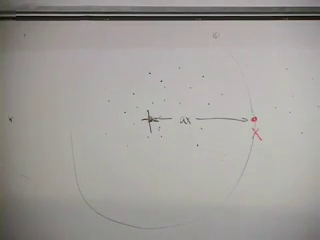
\includegraphics[width=0.70\textwidth]{lecture_08_figure_14.png}
\caption{均匀星系分布、位于共动标记 \(x\) 处的测试星系，以及其径向运动仅由所包围质量控制的球面。}
\lectureframe{01:50:05}
\end{figure}

\begin{figure}[H]
\centering
\begin{tikzpicture}[scale=0.94,>=Latex]
  \draw[gray!65] (0,0) circle (2.35);
  \foreach \p in {
    (-1.5,0.8),(-1.2,-0.8),(-0.8,1.5),(-0.6,0.35),(-0.3,-1.45),
    (0.15,1.05),(0.35,-0.55),(0.7,1.65),(0.9,0.45),(1.25,-0.9),
    (1.65,0.95),(-1.75,-0.2),(1.8,-0.15)} {
    \fill[black!55] \p circle (1.15pt);
  }
  \fill[blue!65!black] (0,0) circle (2pt)
    node[below left] {chosen origin};
  \fill[red!70!black] (2.35,0) circle (2.2pt)
    node[right] {test galaxy};
  \draw[->,thick] (0,0) -- (2.32,0)
    node[midway,above] {\(R=a(t)x\)};
  \draw[<->] (-2.35,-2.55) -- (2.35,-2.55)
    node[midway,below=4pt] {only the enclosed mass contributes};
\end{tikzpicture}
\caption{对壳层定理设置的清晰重建。原点是方便的选择，而不是宇宙的中心。}
\end{figure}

因此，宇宙学多体问题已经变成了一个熟悉的一体问题：一个抛射体在它当前球面内所包含质量的吸引下沿径向运动。牛顿方程将决定\(R=a x\)、从而\(a(t)\)如何加速。讲座有意在完成该计算之前停下。下一次会议将推导最简单的物质主导宇宙学，而不是把答案偷偷塞进几何设定中。

\section{迟来的问题：光、大爆炸与曲率}

正式讲座已经结束，但最后的问题揭示了几幅误导性的图像，它们是物理内容的一部分，而不是附录。

\begin{classroomqa}
\audiencequestion{如果来自极遥远天体的光是在宇宙小得多的时候发出的，为什么它现在看起来来自如此遥远的地方？而如果早期宇宙是致密的，为什么它并非全部可观测？}
\lecturerresponse{必须在膨胀坐标中求解零测地线方程。当\(a(t)\)非常小时，\(dx/dt=1/a(t)\)非常大：光在局域仍以\(c=1\)运动的同时，跨越了很大的共动间隔。随着\(a(t)\)增大，它的共动坐标速度减小。精确的发射点和可观测区域的大小取决于\(a(t)\)的整个历史，因此数值答案要等到某个具体宇宙学被求解之后才能给出。}
\end{classroomqa}

\begin{figure}[H]
\centering
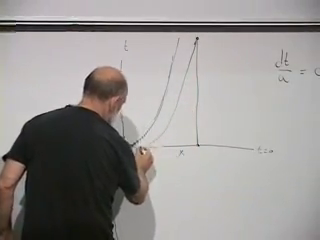
\includegraphics[width=0.72\textwidth]{lecture_08_figure_15.png}
\caption{\((x,t)\)平面中的一条光线：当\(a(t)\)很小时，在共动坐标中近乎水平，随后随着尺度因子增大而逐渐变陡。}
\lectureframe{01:56:20}
\end{figure}

对\eqref{eq:null-ray}积分使被推迟的计算变得明确：
\begin{equation}
  \Delta x
  =\int_{t_{\mathrm e}}^{t_0}\frac{dt}{a(t)}.
  \label{eq:comoving-light-distance}
\end{equation}
当\(t_{\mathrm e}\)趋近于开端时，该积分是否达到任意大的共动距离，取决于\(a(t)\)在早期时间的形式。\editorialnote{方程\eqref{eq:comoving-light-distance}是黑板方程\(dx=dt/a(t)\)的积分形式。它明确给出了讲座留给下一次会议、且尚未选择特定尺度因子的计算。}

\begin{figure}[H]
\centering
\begin{tikzpicture}[scale=0.92,>=Latex]
  \draw[->] (0,0) -- (6.4,0) node[right] {\(x\)};
  \draw[->] (0,0) -- (0,4.6) node[above] {\(t\)};
  \draw[thick,blue!65!black]
    plot[smooth] coordinates {(0,0.18) (1.65,0.42) (2.65,1.05)
      (3.35,2.05) (3.85,3.25) (4.05,4.25)};
  \fill[red!70!black] (4.05,4.25) circle (2pt)
    node[right] {reception today};
  \draw[dashed] (4.05,0) -- (4.05,4.25);
  \node[align=left] at (1.65,3.25)
    {\(\displaystyle \frac{dx}{dt}=\frac1{a(t)}\)\\
     large when \(a\) is small};
\end{tikzpicture}
\caption{共动坐标中光线构造的清晰版本。斜率的改变是坐标效应，而不是局域光速的改变。}
\end{figure}

\begin{classroomqa}
\audiencequestion{大爆炸是否从一个点抛射出物质，因此它现在应当位于一个膨胀的壳层或环上？}
\lecturerresponse{不。该模型始于一个均匀且极其致密的空间。每一个大尺度间隔都在增长；物质并不是从一个优先中心穿过预先存在的空虚空间被发射出去的。均匀布满圆点的气球是一个有用的二维类比：当它膨胀时，所有圆点间隔都增大，而表面仍保持均匀布点。空间甚至在每一个正时刻都可能是无限的；膨胀并不意味着它起初是某个别的东西内部的一个有限球。}
\end{classroomqa}

\begin{classroomqa}
\audiencequestion{在膨胀期间，引力本身是更弱还是更强？}
\lecturerresponse{讨论保持牛顿常数\(G\)固定。尽管如此，力仍会变化，因为间隔和所包含的密度会变化。更早时，同一个共动星系在物理上更近，均匀物质也更致密，因此引力减速更大。这正是壳层定理计算所要量化的内容。}
\end{classroomqa}

最后，空间曲率不可与膨胀相混淆。地球的一小块区域看起来是平的，因为其尺寸与地球半径相比极小。通过测量足够大的三角形，人们要么能探测到角盈余，要么能给出曲率半径的下界。天文学用巨大的三角形做类似的实验。在2006年讲座所用的观测语言中，在可见区域内没有探测到曲率，因此任何曲率半径都必须显著大于该区域。这并不证明宇宙恰好平坦；它限定了可及部分能有多弯曲。

对于球面，内禀曲率按\(R^{-2}\)标度。因此，一个膨胀的球面在局域上变得更平。同样，如果一个均匀宇宙具有非零空间曲率，膨胀会增大其曲率半径，并减小任何固定大小局域斑块中可见的曲率。
\editorialnote{\(R^{-2}\)标度是讲座中“数值曲率随着球面增大而减小”这一陈述的标准定量形式。}

\begin{classroomqa}
\audiencequestion{如果空间是弯曲的，宇宙是否必须有一部分在收缩而另一部分在膨胀？}
\lecturerresponse{不。正、零或负的空间曲率描述的是每一个宇宙时间切片上的几何。膨胀或收缩由\(a(t)\)的演化控制。一个弯曲的宇宙可以膨胀；一个平坦的宇宙可以收缩。膨胀之后可能逆转，正如向上运动的抛射体可能落回，但同时发生的收缩并不隐藏在曲率之中。动力学问题在于，向外的运动究竟是逃脱了所包围质量的吸引、落回，还是恰好位于临界边界上。}
\end{classroomqa}

那个逃逸速度的比较是本讲最后一个板书层面的想法。几何已经提供了度规、哈勃定律和光线方程。牛顿定理已经把动力学归结为一个球体内的质量。下一讲恰好从本讲应当结束的地方开始：从决定\(a(t)\)的方程开始，并从膨胀究竟是逃脱、再坍缩，还是恰好处于刀刃边缘这一问题开始。
